\section{Deep Learning}

\noindent Wie bereits im vorherigen Kapitel erwähnt, bieten künstliche neuronale Netze die Möglichkeit, komplexe Zusammenhänge in Daten zu erkennen. Um diese Fähigkeit zu erlangen, müssen die Netze jedoch erst gebaut werden. Dies geschieht durch die Bildung neuer Schichten und die Anpassung der Gewichte der einzelnen Neuronen. Zu den frühen Zeiten der künstlichen Intelligenz, wurden neuronale Netze von Menschen wie Algorithmen aufgebaut, was nicht nur die Komplexität der Netze begrenzte, sondern voraussetzte, dass die Entwickler den Lösungsweg mathematisch beschreiben konnten. Besonders bei Themen, wie der Erkennung von Sprache und Gesichtern, die vom Gehirn intuitiv erledigt werden, erwies sich dies als sehr schwer. Deshalb wurde der Prozess des \textit{Deep Learnings} entwickelt. Hier soll das neuronale Netz nicht manuell gebaut werden müssen, sondern baut sich selbst, ähnlich wie es das menschliche Gehirn tut. Um dies zu erreichen, muss das Netz trainiert werden. Hierfür wird eine Sammlung von Ein- und Ausgangswertpaaren an die KI gefüttert, welche anschließend die Gewichte so anpasst, dass die Ausgabe des Netzes möglichst nahe an der gewünschten Ausgabe liegt. Dieser Vorgang wird als \textit{Backpropagation} bezeichnet. Die Differenz zwischen der gewünschten und der tatsächlichen Ausgabe wird berechnet und auf die Gewichte der einzelnen Neuronen zurückgeführt. Die Gewichte werden dann so angepasst, dass die Differenz zwischen gewünschter und tatsächlicher Ausgabe minimiert wird. Dieser Vorgang wird so lange wiederholt, bis die Differenz zwischen gewünschter und tatsächlicher Ausgabe minimal ist. Durch diesen Prozess entstehen eine oder mehrere sogenannte \textit{hidden layers}, abstrakte Schichten, welche die Ein- und Ausgangsschichten miteinander verbinden und die Daten in immer abstraktere Formen umwandeln. Die Anzahl der hidden layers und die Anzahl der Neuronen in diesen Schichten sind frei wählbar. Je mehr hidden layers und Neuronen vorhanden sind, desto komplexere Zusammenhänge können erkannt werden. Dieser Prozess wird in Abbildung \ref{fig:deep_learning} dargestellt.\cite{dlbook}\\

\begin{figure}[H]
    \centering
    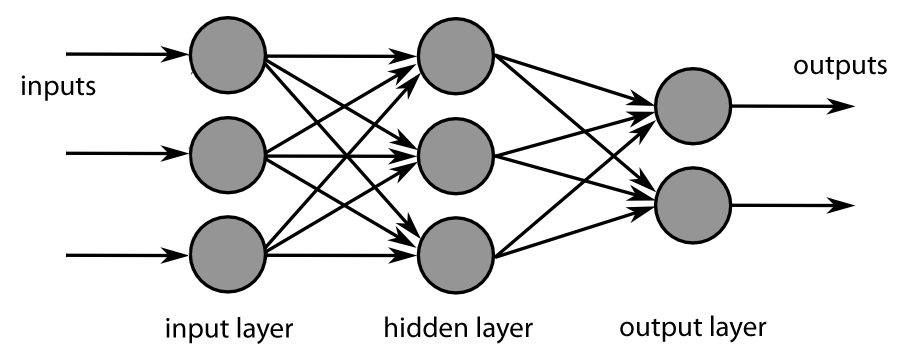
\includegraphics[width=0.6\textwidth]{MultiLayerNeuralNetworkBigger_english.png}
    \caption{Beispiel für neuronales Netz mit einer „hidden layer“} \quelle\url{http://commons.wikimedia.org}
\label{fig:deep_learning}
\end{figure}

\newpage

\noindent Deep Learning ist eine Unterkategorie des Machine Learnings und wird auch als \textit{hierarchisches Lernen} bezeichnet, da die Daten in immer abstraktere Formen umgewandelt werden. Dabei ist der Oberbegriff Machine Learning als solches nicht nur auf neuronale Netze beschränkt, sondern kann auch auf andere Technologien angewendet werden, wie zum Beispiel auf Entscheidungsbäume, Bayes-Netze oder Support Vector Machines. Von Deep Learning wird allerdings nur gesprochen, wenn neuronale Netze verwendet werden. Der Name „Deep Learning“ stammt dabei von der Tiefe der verborgenen \textit{hidden layers}.\\

\noindent Der Prozess des Deep Learnings ist sehr rechenintensiv und benötigt eine große Menge an Trainingsdaten, die in der Regel manuell ausgewählt werden und vorsichtig administriert werden müssen. Zudem ist die Trainingsphase sehr langwierig und kann je nach Größe des Netzes und der Anzahl der Trainingszyklen mehrere Stunden oder sogar Tage dauern. Die Anwendungsphase hingegen ist sehr performant und kann in Echtzeit erfolgen. Der eigentliche Prozess des Deep Learnings ist dabei nicht neu, sondern wurde bereits in den 1980er Jahren entwickelt. Damals scheiterte die Technologie jedoch an der mangelnden Rechenleistung der Computer und der geringen Menge an Trainingsdaten. Erst durch die Entwicklung von leistungsstarken Grafikkarten und die Verfügbarkeit großer Datenmengen, wie sie zum Beispiel im Internet zu finden sind, wurde Deep Learning zu einer praktikablen Technologie. \\

\noindent Durch die Fähigkeit aus großen Datensätzen komplexe Zusammenhänge zu erkennen, ist Deep Learning gut für die Replikation abstrakter Prozesse geeignet, für welche sich das Entwickeln eines klassischen Algorithmus als schwierig herrausstellt. Besonders wenn die Daten sehr komplex sind und große Datensätze für das Training verfügbar sind. Exzellente Beispiele für den Einsatz von Deep Learning wären zum Beispiel die Erkennung von Sprache und Gesichtern. Solche Technologien sind dabei schon weitläufig in Anwenderendgeräten im Einsatz, wie beispielsweise in Form von virtuellen Assistenten, die die Sprache des Anwenders verstehen können oder Kamera-Apps, die die Motive und Gesichter auf Fotos erkennen und anhand dessen klassifizieren. Aber auch in der Medizin und der Biologie wird Deep Learning eingesetzt, um zum Beispiel Krebszellen zu erkennen oder die Struktur von Proteinen zu analysieren. Auch in der Robotik wird Deep Learning eingesetzt, um Roboter zu entwickeln, die sich selbstständig bewegen können. \\

\newpage